\let\negmedspace\undefined
\let\negthickspace\undefined
%\RequirePackage{amsmath}
\documentclass[journal,12pt,twocolumn]{IEEEtran}
 \usepackage[utf8]{inputenc}
 \usepackage{graphicx}
 \usepackage{amsmath}
 \usepackage{mathrsfs}
\usepackage{txfonts}
\usepackage{stfloats}
\usepackage{bm}
\usepackage{cite}
\usepackage{cases}
\usepackage{subfig}
 \usepackage{amsfonts}
 \usepackage{amssymb}
 \usepackage{enumitem}
\usepackage{mathtools}
\usepackage{tikz}
\usepackage{circuitikz}
\usepackage{verbatim}
\usepackage[breaklinks=false,hidelinks]{hyperref}
\usepackage{listings}
\usepackage{calc}
\usepackage{float}
\usepackage{longtable}
\usepackage{multirow}
\usepackage{multicol}
\usepackage{color}
\usepackage{array}
\usepackage{hhline}
\usepackage{ifthen}
\usepackage{chngcntr}

\newcommand{\BEQA}{\begin{eqnarray}}
\newcommand{\EEQA}{\end{eqnarray}}
\newcommand{\define}{\stackrel{\triangle}{=}}
\bibliographystyle{IEEEtran}
%\bibliographystyle{ieeetr}
\def\inputGnumericTable{}
\let\vec\mathbf
\providecommand{\pr}[1]{\ensuremath{\Pr\left(#1\right)}}
\providecommand{\cdf}[2]{\ensuremath{F_{#1}\left(#2\right)}}
\providecommand{\sbrak}[1]{\ensuremath{{}\left[#1\right]}}
\providecommand{\lsbrak}[1]{\ensuremath{{}\left[#1\right.}}
\providecommand{\rsbrak}[1]{\ensuremath{{}\left.#1\right]}}
\providecommand{\brak}[1]{\ensuremath{\left(#1\right)}}
\providecommand{\lbrak}[1]{\ensuremath{\left(#1\right.}}
\providecommand{\rbrak}[1]{\ensuremath{\left.#1\right)}}
\providecommand{\cbrak}[1]{\ensuremath{\left\{#1\right\}}}
\providecommand{\lcbrak}[1]{\ensuremath{\left\{#1\right.}}
\providecommand{\rcbrak}[1]{\ensuremath{\left.#1\right\}}}
%\providecommand{\abs}[1]{\left\vert#1\right\vert}
\providecommand{\res}[1]{\Res\displaylimits_{#1}}
\newcommand{\myvec}[1]{\ensuremath{\begin{pmatrix}#1\end{pmatrix}}}
\newcommand{\mydet}[1]{\ensuremath{\begin{vmatrix}#1\end{vmatrix}}}
\newcommand{\PROBLEM}{\noindent \textbf{PROBLEM: }}
\newcommand{\solution}{\noindent \textbf{Solution: }}
\newcommand{\note}{\noindent \textbf{Note: }}
\newcommand{\tofind}{\noindent \textbf{To find: }}
\title{Assignment 5}
\author{MANIKANTA UPPULAPU\\BT21BTECH11005}
\date{}
\begin{document}
% make the title area
\maketitle
\PROBLEM Three letters are dictated to three persons and an envelope is addressed to each of them, the letters are inserted into the envelopes at random so that each envelope contains exactly one letter. Find the probability that at least one letter is in its proper envelope.\\

\solution Let $X$ be a random variable denote the number of letters properly inserted into correct envelope.we can see that the sample space $S = \cbrak{0,1,2}$. \\
The PMF is given by
\begin{equation}
\pr{X = k} = 
\begin{cases}
\frac{2}{6}, & k=0\\
\frac{3}{6}, & k=1\\
\frac{1}{6}, & k=2\\
0, & \text{otherwise} 
\end{cases}
\label{pmf}
\end{equation}
\noindent The CDF can be derived from the PMF as follows:
\begin{align}
\cdf{X}{k} = \pr{X \leq k}  &= \sum_{i = 1}^{i = k}\pr{X = i} 
\label{eqn:cdf}
\end{align}
\noindent Therefore, the CDF is explicitly given by
\begin{equation}
\cdf{X}{k} = 
\begin{cases}
\frac{2}{6}, & k=0\\
\frac{5}{6}, & k=1\\
1, & k \geq 2
\end{cases}
\label{cdf}
\end{equation}
\noindent Hence, using \autoref{fig:pmf-cdf},
\begin{align}
\pr{X=0} &= \cdf{X}{0} = \frac{2}{6} = \frac{1}{3}  \\
\implies \pr{X \geq 1} &= 1 - \cdf{X}{0} \\
&= 1 - \frac{1}{3} = \frac{2}{3} 
\label{sol}
\end{align}

\begin{figure}[!ht]
\centering
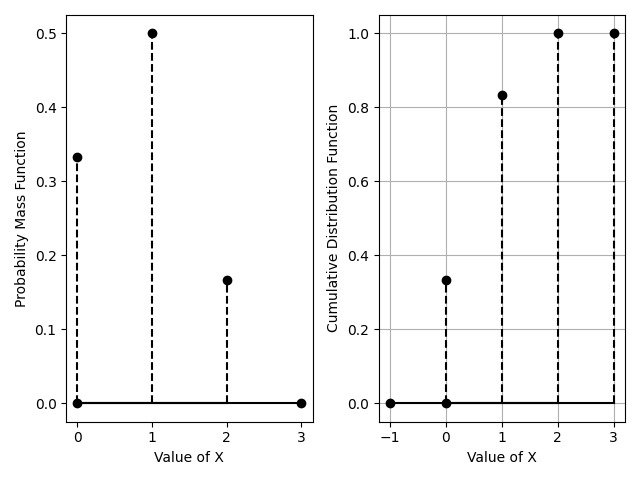
\includegraphics[width=\columnwidth]{fig1.jpeg}
\caption{Plot of the PMF (left) and CDF (right). Code: \texttt{codes/assign{\_}5.py}}
\label{fig:pmf-cdf}
\end{figure}

\end{document}
